\documentclass[11pt]{article}
\usepackage[margin=0.8in]{geometry}
\usepackage[T1]{fontenc}
\usepackage{lmodern,microtype,booktabs,graphicx,amsmath,xcolor,hyperref,xurl}
\hypersetup{colorlinks=true,urlcolor=blue,linkcolor=blue,pdftitle={What one additional river gauge changes},pdfauthor={James N. Jean IV}}
\setlength{\parindent}{0pt}\setlength{\parskip}{6pt}\setlength{\tabcolsep}{5pt}
\newcommand{\SourceRows}{14,864}
\newcommand{\QualifiedRows}{1,421}
\newcommand{\SourceGates}{40}
\newcommand{\LocalSkill}{15.32}
\newcommand{\PairSkill}{28.96}
\newcommand{\SkillDifference}{13.64}
\newcommand{\DevChecks}{216,162}
\newcommand{\FinalChecks}{831,539}
\newcommand{\FinalPredictions}{59,154}
\newcommand{\PanelCount}{192}
\newcommand{\TrentonApproval}{64}
\newcommand{\WinonaApproval}{322}
\newcommand{\MuscodaApproval}{335}
\newcommand{\ThreeLocal}{0.1}
\newcommand{\ThreePair}{0.01}
\newcommand{\OneLocal}{0.1}
\newcommand{\OnePair}{0.001}
\newcommand{\MissADays}{365}
\newcommand{\MissABaseMse}{0.025204}
\newcommand{\MissALocalMse}{0.022532}
\newcommand{\MissAPairMse}{0.016165}
\newcommand{\MissALocalCfsMse}{81.55}
\newcommand{\MissAPairCfsMse}{46.22}
\newcommand{\MissBDays}{366}
\newcommand{\MissBBaseMse}{0.024929}
\newcommand{\MissBLocalMse}{0.021077}
\newcommand{\MissBPairMse}{0.017260}
\newcommand{\MissBLocalCfsMse}{64.77}
\newcommand{\MissBPairCfsMse}{39.50}
\newcommand{\SusADays}{365}
\newcommand{\SusABaseMse}{0.135273}
\newcommand{\SusALocalMse}{0.114212}
\newcommand{\SusAPairMse}{0.106492}
\newcommand{\SusALocalCfsMse}{403.45}
\newcommand{\SusAPairCfsMse}{416.16}
\newcommand{\SusBDays}{366}
\newcommand{\SusBBaseMse}{0.185627}
\newcommand{\SusBLocalMse}{0.149136}
\newcommand{\SusBPairMse}{0.133763}
\newcommand{\SusBLocalCfsMse}{999.91}
\newcommand{\SusBPairCfsMse}{929.53}
\newcommand{\ReplayExact}{1,079,126}
\newcommand{\ReplayNumeric}{298,395}
\begin{document}
\begin{center}{\LARGE\bfseries What one additional river gauge changes}\par
\vspace{5pt}{\large A retrospective daily-discharge prediction exercise}\par
James N. Jean IV \quad | \quad Independent research program, Study 14 v2\par
October 30, 2026 \quad | \quad Not peer reviewed
\end{center}
\section*{The decision}
Before paying to operate another monitoring feed, establish whether it improves the question being asked. This study compares the target gauge's own history with the same history plus one additional gauge, under fixed date lags and a synthetic input outage. It tests prediction information in supplied records. It does not price a gauge, select an optimal network or validate a flood warning.

\textbf{Finding under the declared log-flow objective.} Across four final basin/year panels, the equal-panel mean skill versus persistence is \PairSkill{}\% for the pair model and \LocalSkill{}\% for local history alone. The difference is \SkillDifference{} percentage points of persistence-normalized log MSE. The pair model has lower log MSE in each primary panel. Training and configuration selection use earlier years; no final score changes a setting.

\textbf{The error scale matters.} In Susquehanna 2023, the pair model has lower log MSE but \emph{higher} MSE in cubic-feet-per-second units: \SusAPairCfsMse{} versus \SusALocalCfsMse{} million cfs$^2$. This is not a win on every loss or physical scale. The choice of objective must reflect the decision, particularly when high-flow errors matter.

\textbf{Practical recommendation.} Take the specific gauge pair into a prospective source-availability and error-cost pilot before selecting an operational model or funding a monitoring change. Keep local history and persistence in the comparison. The offline review command checks that models share target dates and displays both log and cfs MSE so a favorable transformed-scale result cannot hide the other measure.

\textbf{Why this is version 2.} The original 2020--2025 source gate failed because three 2025 station-years lacked sufficient Approved days. That failure remains intact. This separately specified analysis uses 2020--2024, informed by the existing approval ledger before any modelling. It keeps the same eight gauges and 95\% approval threshold, with a revised temporal split. It does not certify that version 1 passed.

\textbf{Scope.} These are later Approved daily discharge records under synthetic date lags. They do not establish what was available on an actual historical forecast date. No measured operational lead time, outage frequency, safety outcome, deployment benefit, causal effect or financial saving follows.

\clearpage
\section*{1. Source and the visible redesign}
The official USGS daily-values API supplies Primary Daily Mean discharge: parameter 00060, statistic 00003, in cubic feet per second (cfs). Complete original responses, monitoring-location records and matching before/after time-series metadata were retained privately. The public package contains selected factual date/value/unit/approval/qualifier cells, minimal station/series metadata and exact response hashes. USGS-produced factual data may be reused with acknowledgment; third-party agency artwork and complete documents are excluded.

Version 1 captured 17,784 rows from December 2019 through December 2025. Its fixed 95\% usable Approved-day gate failed in 2025: Trenton had \TrentonApproval{}/365 days, Winona \WinonaApproval{}/365 and Muscoda \MuscodaApproval{}/365. The 374 Provisional records were not relabelled, interpolated into compliance or treated as original real-time observations. The original protocol and failure receipt remain public; complete original captures and the first unvalidated projection remain private.

\textbf{V2 source boundary.} The redesign was committed at \texttt{1e498c6e3d0b} before any recorded-data model fit. It reuses the exact captures, taking December 2019 as feature warm-up and 2020--2024 as the analysis period. This approval-informed choice is an acknowledged source-selection limitation, not a blinded collection or external preregistration. No model error or correlation informed it. All source values were already present.

V2 has \SourceRows{} usable Approved rows including warm-up, with all \SourceGates{} station-year gates passing. Every station/year has complete daily support in this slice. The \QualifiedRows{} rows with nonempty qualifiers, including estimated flags, remain in the primary analysis. A fixed sensitivity excludes a target date when its label or any required input has a nonempty qualifier; the fitted models stay unchanged. Missing records are never imputed.

\begin{center}\small
\begin{tabular}{lll}\toprule
Basin & Target gauge & Additional gauge\\\midrule
Wisconsin & 05407000 & 05400760\\
Delaware & 01463500 & 01457500\\
Susquehanna & 01576000 & 01570500\\
Mississippi & 05420500 & 05378500\\\bottomrule
\end{tabular}\end{center}

\textbf{Split.} Train on 2020--2021. Select configurations using Wisconsin/Delaware validation in 2022. Evaluate 2023--2024 in Susquehanna/Mississippi as the four primary panels, retaining the development basins' later results as context. The held basins may fit their own coefficients on 2020--2021 after selection is frozen. This is geographic separation for configuration selection, not transfer of one fitted model to a never-seen basin. River labels alone do not establish causal connectivity or travel time.

\clearpage
\section*{2. Fixed features, baselines and selection}
Define $z(d)=\log(1+Q(d)/(1\ \mathrm{cfs}))$. Primary lag $L=3$ days and sensitivity $L=1$ use no measurement dated after $d-L$. Persistence predicts $z(d-L)$. Both ridge models predict its residual $z(d)-z(d-L)$. Local features are the lagged target level, one-day and seven-day differences, and target-date sine/cosine seasonality with period 365.25 days and January 1 phase zero. The pair adds the additional gauge's same three lagged level/change features. Both families use identical complete training dates and training-only population means/scales; a zero scale becomes 1 and is flagged.

The response intercept is unpenalized. With standardized training design $X$, the objective is mean squared residual error plus $\lambda\|\beta\|_2^2$, so its normal matrix is $X^\top X+n\lambda I$. The fixed grid is $\{0.001,0.01,0.1,1\}$. Each family/lag selects its penalty by equal-basin validation log MSE. Values within absolute $10^{-12}$ of the minimum tie in favor of larger $\lambda$. There is no validation refit or grid extension. Final predicted $z$ is clipped below at zero before the inverse transform to cfs.

\begin{center}\small\begin{tabular}{rlr}\toprule
Lag (days) & Family & Selected $\lambda$\\\midrule
3 & local & \ThreeLocal{} \\
3 & pair & \ThreePair{} \\
1 & local & \OneLocal{} \\
1 & pair & \OnePair{} \\
\bottomrule\end{tabular}\end{center}
\begin{center}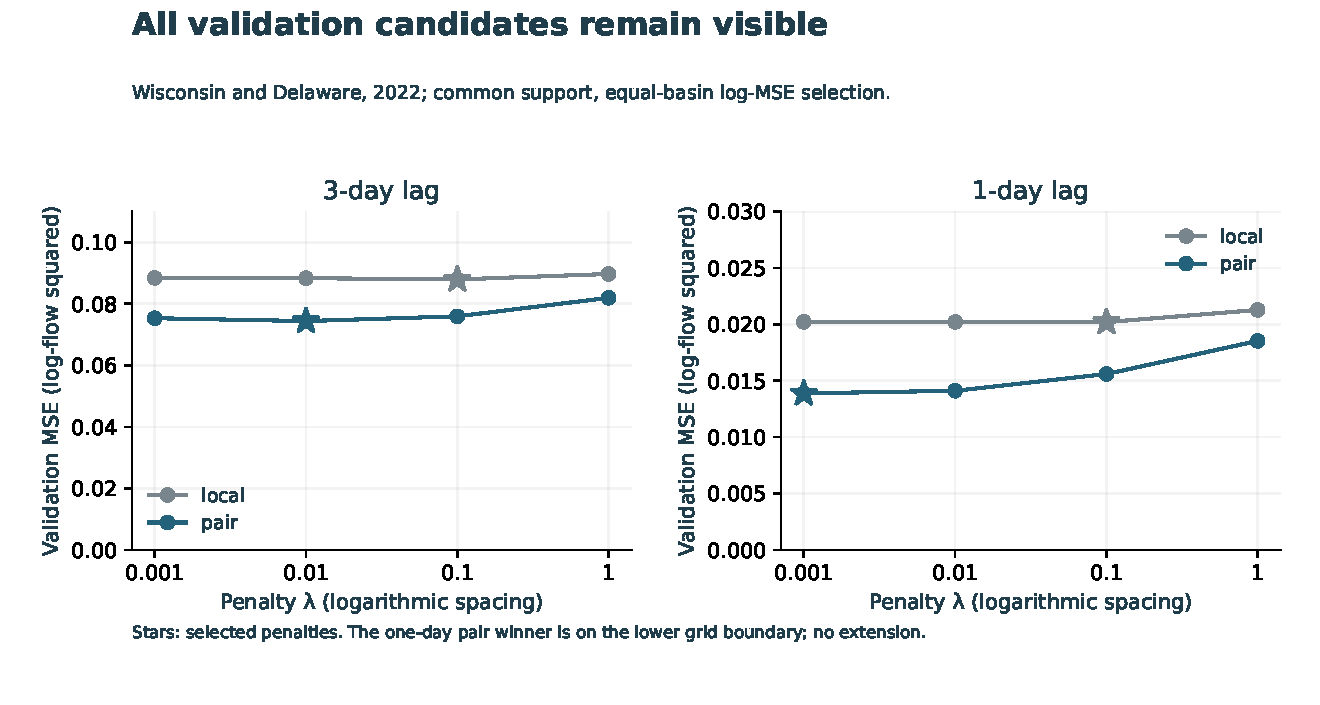
\includegraphics[width=\linewidth]{images/gauge_validation.pdf}\end{center}
All 32 development fits, 36 fold scores including persistence, 16 equal-basin objectives and 13,140 validation predictions remain visible. The one-day pair model selects the grid's lower boundary; it is not a demonstrated global optimum. Thirty-four source, protocol, code, fixture and development dependencies were committed and frozen at \texttt{085b5a545fe8} before any final scores.

\clearpage
\section*{3. Final comparison on the declared objective}
For each common-support panel, $\mathrm{skill}=1-\mathrm{MSE}_{model}/\mathrm{MSE}_{persistence}$ in log-flow units. The final equal-panel mean gives four panels equal weight rather than pooling their dependent days. All source labels, dates, fitted coefficients, preprocessing and selected penalties stay fixed.
\begin{center}\small\begin{tabular}{lrrrr}\toprule
Primary panel & Days & Persistence MSE & Local MSE & Pair MSE\\\midrule
Mississippi 2023 & \MissADays{} & \MissABaseMse{} & \MissALocalMse{} & \MissAPairMse{} \\
Mississippi 2024 & \MissBDays{} & \MissBBaseMse{} & \MissBLocalMse{} & \MissBPairMse{} \\
Susquehanna 2023 & \SusADays{} & \SusABaseMse{} & \SusALocalMse{} & \SusAPairMse{} \\
Susquehanna 2024 & \SusBDays{} & \SusBBaseMse{} & \SusBLocalMse{} & \SusBPairMse{} \\
\bottomrule\end{tabular}\end{center}
\begin{center}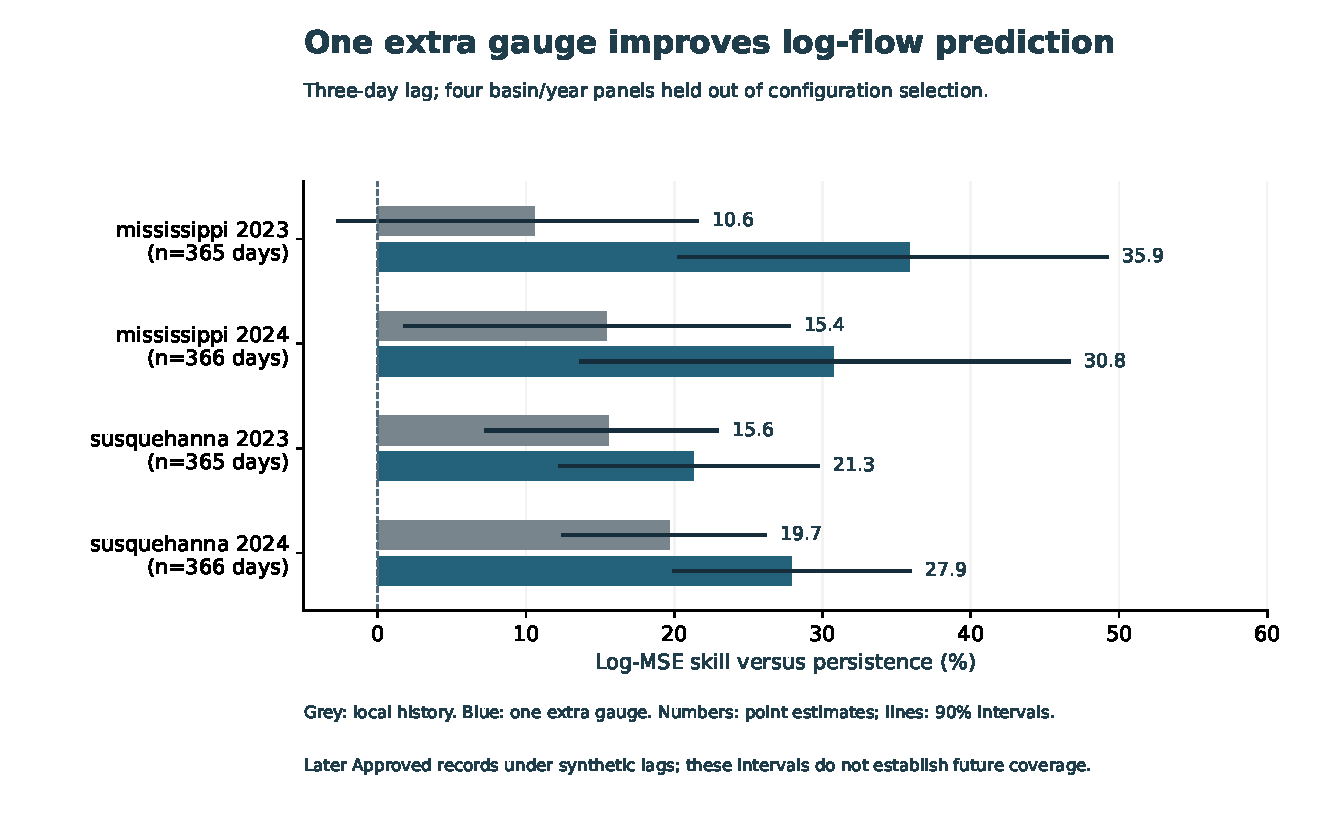
\includegraphics[width=\linewidth]{images/primary_gauge_skill.pdf}\end{center}
Each pair-minus-local conditional 90\% interval is above zero in this finite comparison. The intervals come from 500 circular 14-day paired block replicates per panel, with retained starts and replicate estimates, NumPy PCG64 seed 20261029, and linear 5th/95th percentiles. They describe within-year resampling conditional on these records. Four panels, seasonal dependence, common geography and the approval-informed period prevent a future-year, new-basin or causal coverage claim. No p-value or independent-day assumption is used.

\clearpage
\section*{4. Sensitivity and the physical error scale}
The fixed outage hides additional-gauge inputs on seven of every 28 lagged input dates and routes the pair model to its selected local model. Required additional-gauge records still define common scoring support, so the scenario cannot improve a score by silently discarding difficult dates. This is a synthetic fallback, not observed telemetry behavior.
\begin{center}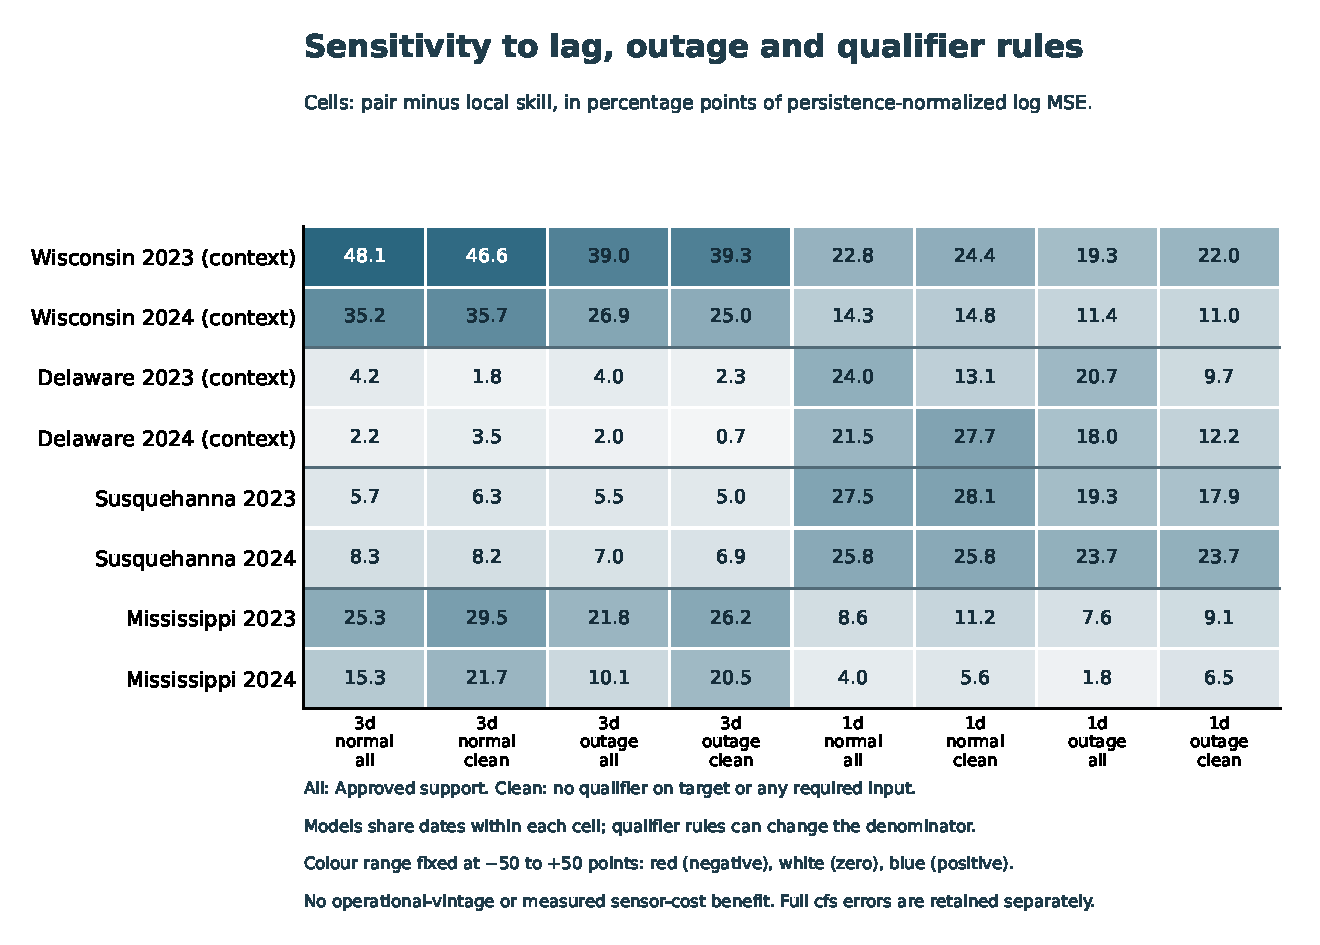
\includegraphics[width=\linewidth]{images/gauge_sensitivity.pdf}\end{center}
All 64 pair/local sensitivity comparisons favor the pair model in log-MSE skill, with different gains. They are dependent descriptive comparisons, not 64 independent replications. Qualifier rules can change support; every model within one cell uses identical target dates. The complete \PanelCount{} metric rows and \FinalPredictions{} predictions include both units' MAE/MSE/RMSE, cfs signed error, training-mean-normalized cfs RMSE, clipping and fallback counts.
\begin{center}\small\begin{tabular}{lrr}\toprule
Primary panel & Local MSE (million cfs$^2$) & Pair MSE (million cfs$^2$)\\\midrule
Mississippi 2023 & \MissALocalCfsMse{} & \MissAPairCfsMse{} \\
Mississippi 2024 & \MissBLocalCfsMse{} & \MissBPairCfsMse{} \\
Susquehanna 2023 & \SusALocalCfsMse{} & \SusAPairCfsMse{} \\
Susquehanna 2024 & \SusBLocalCfsMse{} & \SusBPairCfsMse{} \\
\bottomrule\end{tabular}\end{center}
Susquehanna 2023 reverses the model ordering on physical-unit MSE. The transformed objective puts a different weight on discharge errors. A recommendation must preserve that distinction and the user's decision cost rather than turn the log-scale result into an unqualified performance claim.

\clearpage
\section*{5. Verification, reproducibility and next evidence}
The native-source checker independently reconciles all selected rows against complete private official responses using separate date/value parsing and SQLite coverage counts. It checks 148,640 native fields, 163,504 projected scalars, 89,184 normalized scalars and 40 station-year coverage totals. Metadata hashes and matching before/after versions are retained. Offline public-source replay checks the saved factual projection and its original hash-bound certificate; it does not reacquire mutable historical API responses.

The analytical checker imports no production feature, fit, prediction, metric or selector helpers. Separate SQLite date joins reconstruct the common support and features. Augmented-design least-squares SVD checks ridge fits independently of the production normal equations. Scalar forecasts, SQL error aggregates, a separate selector and retained-draw scalar resampling check \DevChecks{} development and \FinalChecks{} final conditions. Twenty-three authored fixture methods and three authored panel-review cases pass. Counts, dates, configurations, routing, random draws and selection are exact. Log-space/dimensionless numerical tolerances are absolute $10^{-8}$; cfs metrics use absolute $10^{-4}$ plus relative $10^{-10}$. These are finite numerical checks, not universal correctness.

Separate full-history clones at analysis revision \texttt{d122d8540bbe} pass complete analysis replays on CPython 3.10.11 and 3.12.14 with NumPy 2.2.5. Each checks \ReplayExact{} exact facts and \ReplayNumeric{} numeric facts with three source files unchanged and no source request. Four as-run discrepancy diagnostics are independently bounded rather than required to match bit-for-bit. The rendered figures separately bind source values, intervals, labels, geometry and heatmap colors. Figure and paper checks supplement the analysis replay; release CI checks the exact final revision.

\textbf{What remains unestablished.} Later Approved daily records cannot demonstrate actual historical publication timing, real forecast lead time, water levels, inundation or flood impacts. Four fixed gauge pairs cannot identify an optimal network. Synthetic outages and retained common support do not estimate a live system's missingness or costs. No deployment, realized resource saving, causal benefit or safety recommendation is claimed. The original v1 failure remains evidence, and v2's period choice must remain visible.

\textbf{Next step.} Fix a decision-relevant loss, capture prospective availability and revision timestamps, and evaluate the local/pair/persistence comparison with actual outage support before operational selection or a monitoring investment. Preserve all present errors and qualify any gain by its scale and denominator.

\small\textbf{Sources and reproducible methods.}\par
USGS Daily Values documentation: \url{https://api.waterdata.usgs.gov/ogcapi/v1/collections/daily}. Provisional-data statement: \url{https://water.usgs.gov/data/provisional.html}. Reuse guidance: \url{https://www.usgs.gov/faqs/are-usgs-reportspublications-copyrighted}. Credit: U.S. Geological Survey. This project selects and transforms factual cells; it does not imply USGS endorsement.\par
NumPy linear algebra documentation, least-squares interface: \url{https://numpy.org/doc/2.2/reference/generated/numpy.linalg.lstsq.html}. Ridge, persistence and block resampling are established methods; no new estimator or comprehensive scientific-priority claim is made.\par
Protocol versions, full outputs, offline exercise and replay: \url{https://github.com/S3R3Bii/gauge-information-budget}. Independent program manuscript; formal-publication projects remain private.
\end{document}
